\section{Experiments}

In this section, we provide empirical results on MNIST dataset to demonstrate the effectiveness of our proposed algorithms. The model we use is the LeNet-5 Convolutional Neural Network (CNN) architecture introduced in~\cite{lecun1998gradient}, with $60\,000$ model parameters in total.

Four methods are compared in our experiments: Federated SGD (FedSGD), SketchSGD~\cite{ivkin2019communication}, FedSketch-PRIVIX (FS-PRIVIX) and FedSketch-HEAPRIX (FS-HEAPRIX). We implement the algorithms by simulating the distributed and federated environment. 
Note that in Algorithm~\ref{Alg:PFLHom}, FS-PRIVIX with global learning rate $\gamma=1$ is equivalent to the DiffSketch algorithm proposed in \cite{li2018federated}. 
In the following experiments, we set the number of workers to $50$. 
For federated learning algorithms, we use different number of local updates $\tau$. 
For SketchedSGD which is under synchronous distributed learning framework, $\tau$ is fixed and equal to $1$. 
For all methods, we tune the learning rates (both local, i.e. $\eta$ and global, i.e. $\gamma$, if applicable) over the log-scale and report the best results.

In each round of local update, we randomly choose half of the local devices to be active, which is the common practice in real-world applications. 
For the data distribution on each device, we test both \emph{homogeneous} and \emph{heterogeneous} setting. 
In the former case, each device receives uniformly drawn data samples (each class has equal probability to be selected). 
In the latter case, each device only receives samples from one or two classes among ten digits in the MNIST dataset. 
Since data is not distributed i.i.d. among local devices, training is expected to be harder in the heterogeneous case.

\begin{figure}[ht]
	\begin{center}
		\mbox{			    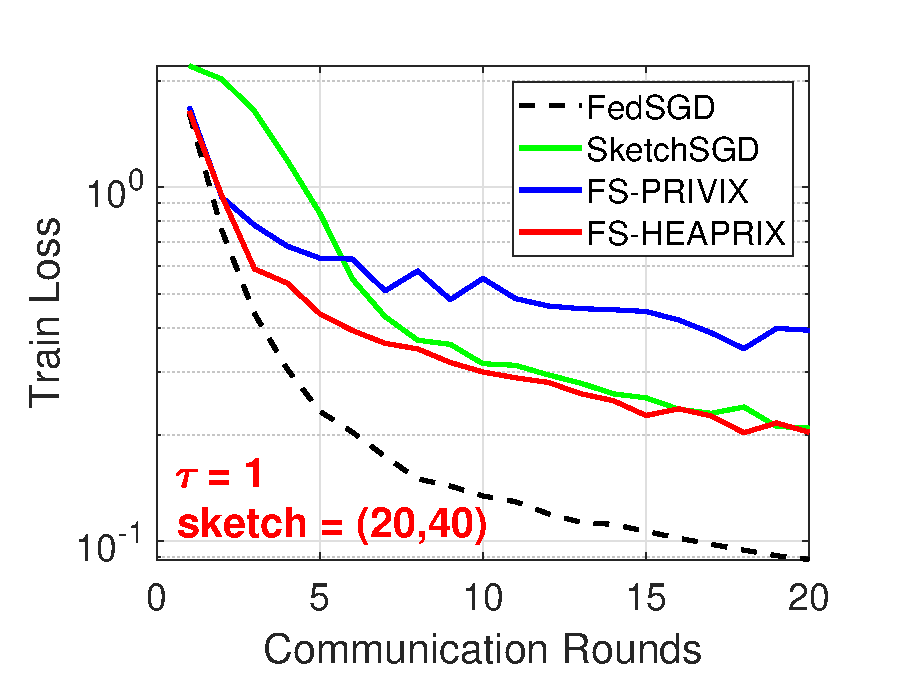
\includegraphics[width=3in]{MNIST_figures/local1_sketch20_iid1_train_loss.eps}
		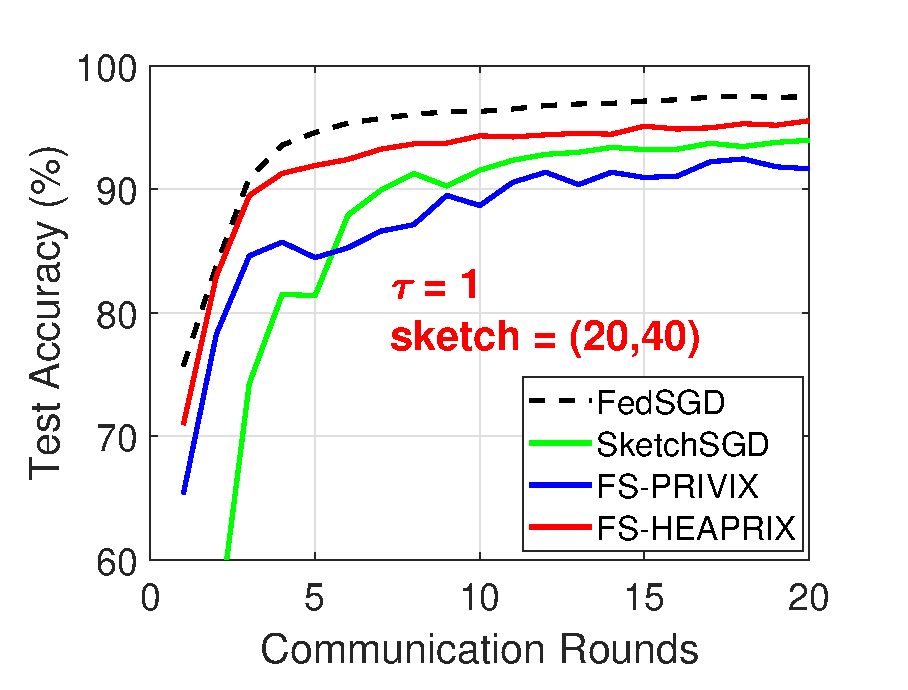
\includegraphics[width=3in]{MNIST_figures/local1_sketch20_iid1_test_acc.eps}
		}
		\mbox{
		\includegraphics[width=3in]{MNIST_figures/local1_sketch50_iid1_train_loss.eps}
		\includegraphics[width=3in]{MNIST_figures/local1_sketch50_iid1_test_acc.eps}
		}
	\end{center}
	\caption{Homogeneous case: Comparison of four algorithms on LeNet CNN architecture.}
    \label{fig:MNIST-tau1}
\end{figure}

\begin{figure}[h]
	\begin{center}
		\mbox{			    \includegraphics[width=1.6in]{MNIST_figures/local2_sketch20_iid1_train_loss.eps}
		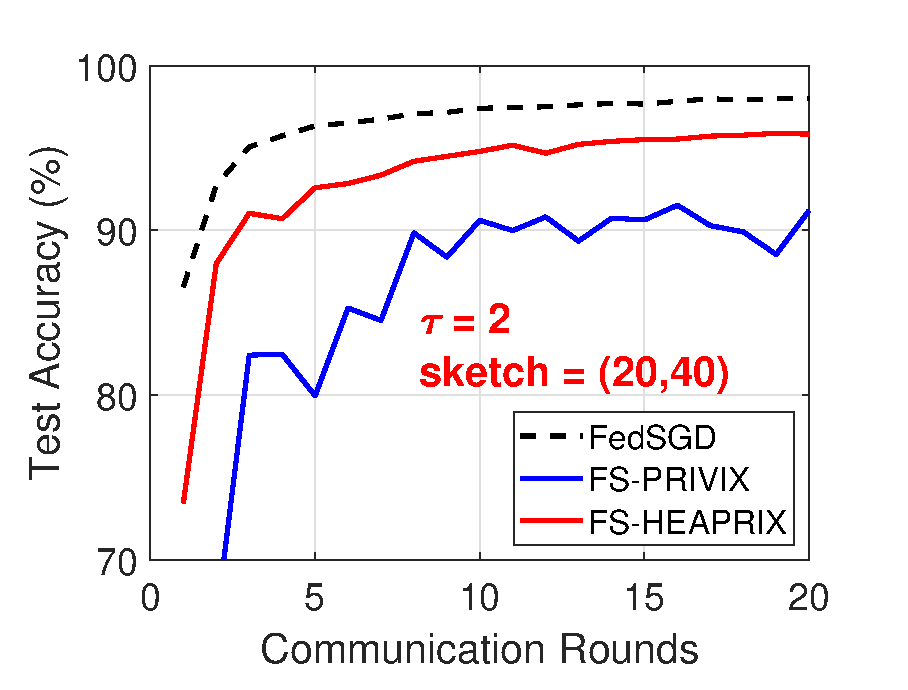
\includegraphics[width=1.6in]{MNIST_figures/local2_sketch20_iid1_test_acc.eps}
		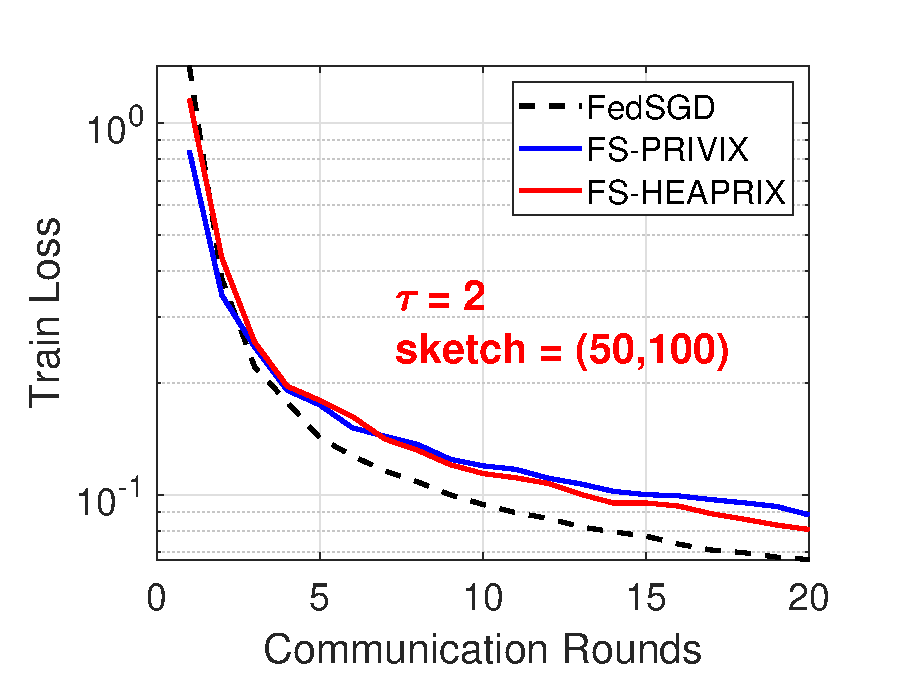
\includegraphics[width=1.6in]{MNIST_figures/local2_sketch50_iid1_train_loss.eps}
		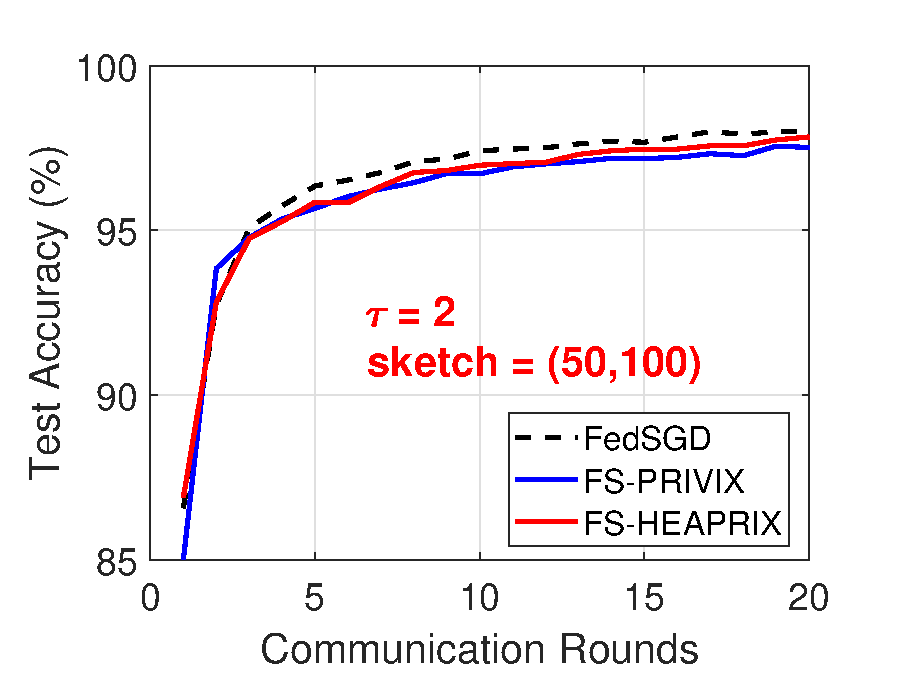
\includegraphics[width=1.6in]{MNIST_figures/local2_sketch50_iid1_test_acc.eps}
		}
		
		\mbox{			    \includegraphics[width=1.6in]{MNIST_figures/local5_sketch20_iid1_train_loss.eps}
		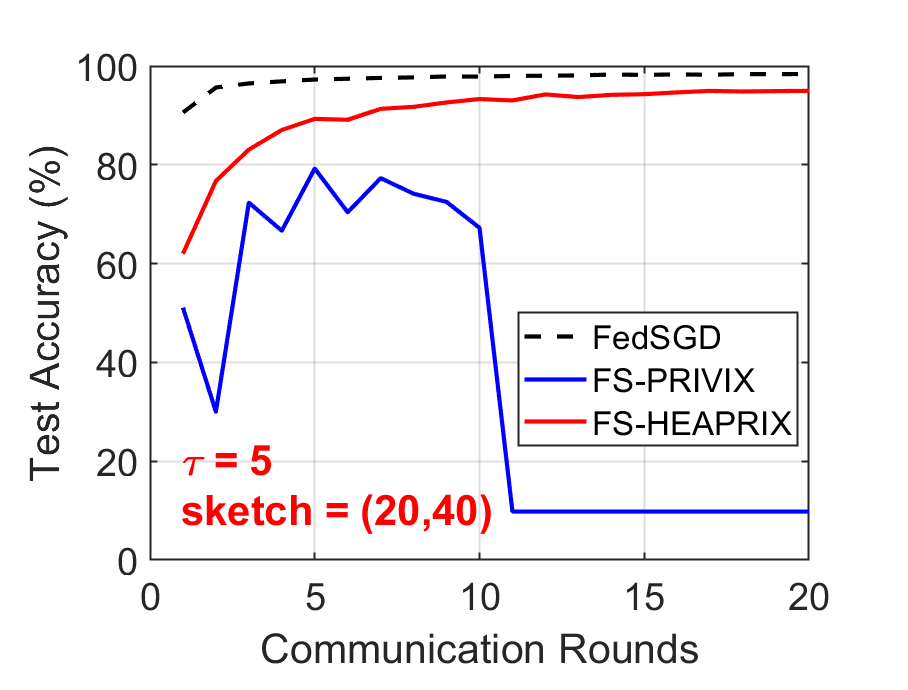
\includegraphics[width=1.6in]{MNIST_figures/local5_sketch20_iid1_test_acc.eps}
		\includegraphics[width=1.6in]{MNIST_figures/local5_sketch50_iid1_train_loss.eps}
		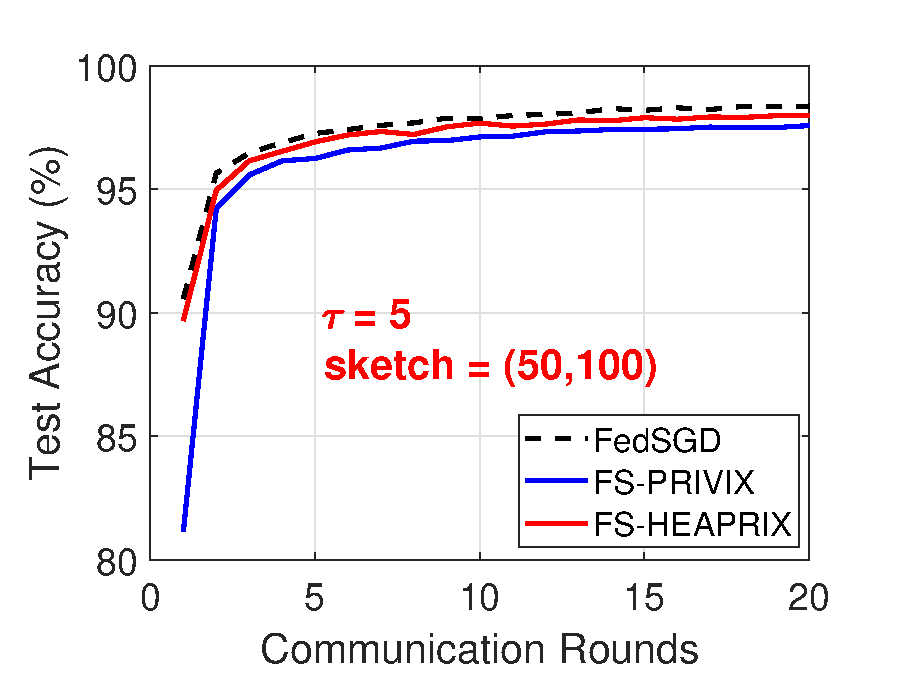
\includegraphics[width=1.6in]{MNIST_figures/local5_sketch50_iid1_test_acc.eps}
		}
	\end{center}
	\caption{Homogeneous case: comparison of FedSGD, FS-PRIVIX and FS-HEAPRIX on LeNet CNN architecture, with number of local updates being 2 and 5.}
    \label{fig:MNIST-tau2,tau5}
\end{figure}


\textbf{Homogeneous case.} In Figure~\ref{fig:MNIST-tau1}, we provide the training loss and test accuracy for the four algorithms mentioned above, with $\tau=1$ (since SketchSGD requires single local update per round). 
We also test different sizes of sketching matrix, $(t,k)=(20,40)$ and $(50,100)$. Note that these two choices of sketch size correspond to a $75\times$ and $12\times$ compression ratio, respectively. 
In general, as one would expect, higher compression ratio leads to worse learning performance. In both cases, FS-HEAPRIX performs the best in terms of both training objective and test accuracy. FS-PRIVIX is better when sketch size is large (i.e. when the estimation from sketches are more accurate), while SketchSGD performs better with small sketch size. 

The results for multiple local updates are given in Figure~\ref{fig:MNIST-tau2,tau5}, where we set $\tau=2,5$. We see that FS-HEAPRIX is significantly better than FS-PRIVIX, either with small or large sketching matrix. In both cases, FS-HEAPRIX yields acceptable extra test error compared to FedSGD, especially when considering the high compression ratio (e.g. $75\times$). However, FS-PRIVIX performs poorly with small sketch size $(20,40)$, and even diverges with $\tau=5$. 
We also observe that the performances of FS-HEAPRIX improve when the number of local updates increases. That is, the proposed method is able to further reduce the communication cost by reducing the number of rounds required for communication. This is also consistent with our theoretical claims established in this paper. For $\tau=1,2,5$, we see that a sketch size of $(50,100)$ is sufficient to give similar test accuracy as the federated SGD (FedSGD).

\textbf{Heterogeneous case.} We plot similar sets of results in Figure~\ref{fig:MNIST-tau1-iid0} and Figure~\ref{fig:MNIST-tau2,tau5-iid0} for non-i.i.d. data distribution (heterogeneous setting). This setting leads to more twists and turns in the training curves. 
From Figure~\ref{fig:MNIST-tau1-iid0} ($\tau=1$), we see that SketchSGD performs very poorly in the heterogeneous case, while both our proposed FedSketchGATE methods, see Algorithm~\ref{Alg:PFLHet}, achieve similar generalization accuracy as the federated SGD (FedSGD) algorithm, even with fairly small sketch size (i.e. $75\times$ compression ratio). In addition, FS-HEAPRIX is again better than FS-PRIVIX in terms of both training loss and test accuracy.

Furthermore, we notice in Figure~\ref{fig:MNIST-tau2,tau5-iid0} the advantage of FS-HEAPRIX over FS-PRIVIX. However, empirically we see that in the heterogeneous setting, more local updates $\tau$ tend to undermine the learning performance, especially with small sketch size. This is because in this scenario, each local device only receives samples with a few classes, so each local model is actually trained with biased stochastic gradients. More local updates would result in more bias in the local models, which makes federated averaging less effective. Nevertheless, we see that when sketch size is large, i.e. $(50,100)$, FS-HEAPRIX can still provide comparable test accuracy as FedSGD.

Our empirical study demonstrates that our proposed FedSketch (and FedSketchGATE) frameworks are able to perform well in homogeneous (resp. heterogeneous) learning setting, with high compression rate. In particular, FedSketch methods are advantageous over prior SketchedSGD~\cite{ivkin2019communication} method in both cases. FS-HEAPRIX performs the best among all the tested compressed optimization algorithms, which in many cases achieves similar generalization accuracy as federated SGD with small sketch size. In general, in any tested case, we can at least achieve $12\times$ compression ratio with very little loss in test accuracy.

\begin{figure}[h]
	\begin{center}
		\mbox{			    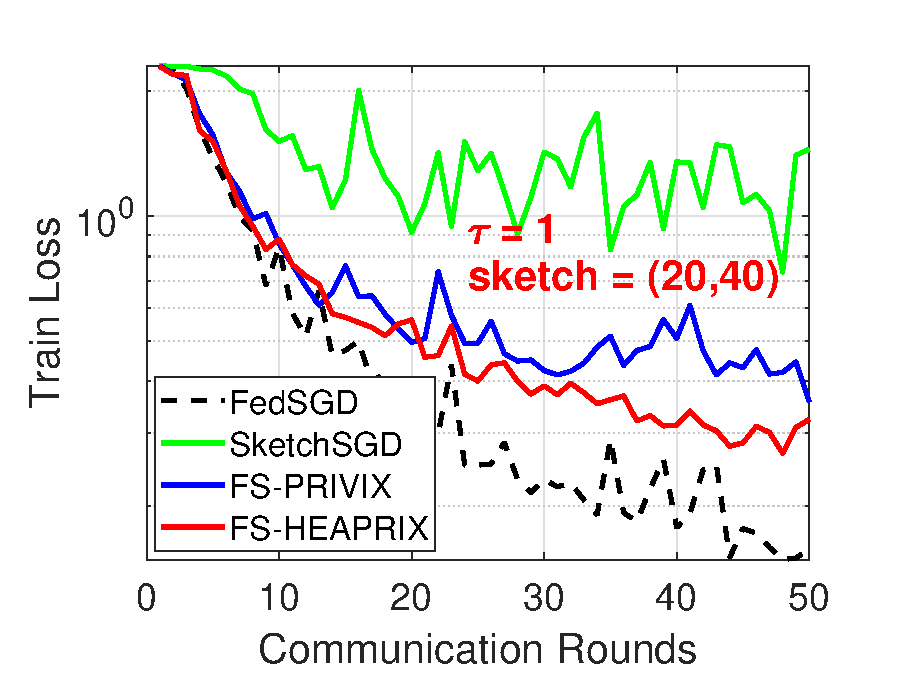
\includegraphics[width=3in]{MNIST_figures/local1_sketch20_iid0_train_loss.eps}
		\includegraphics[width=3in]{MNIST_figures/local1_sketch20_iid0_test_acc.eps}
		}
		\mbox{
		\includegraphics[width=3in]{MNIST_figures/local1_sketch50_iid0_train_loss.eps}
		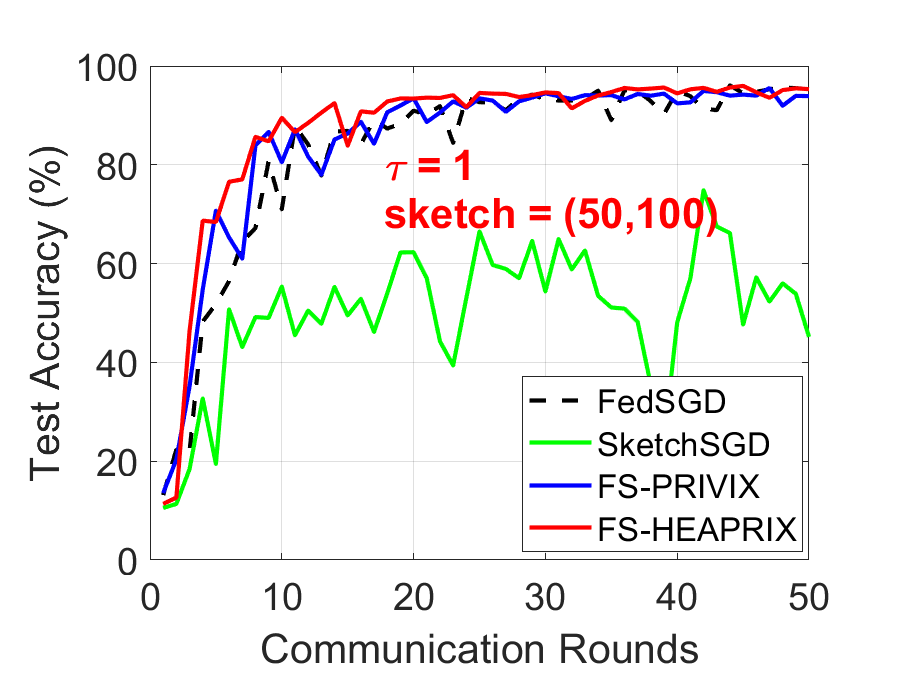
\includegraphics[width=3in]{MNIST_figures/local1_sketch50_iid0_test_acc.eps}
		}
	\end{center}
	\caption{Heterogeneous case: the comparison of four algorithms on LeNet CNN architecture.}
    \label{fig:MNIST-tau1-iid0}
\end{figure}


% \begin{figure}[h]
% 	\begin{center}
% 		\mbox{			    \includegraphics[width=1.6in]{MNIST_figures/local2_sketch20_iid0_train_loss.eps}
% 		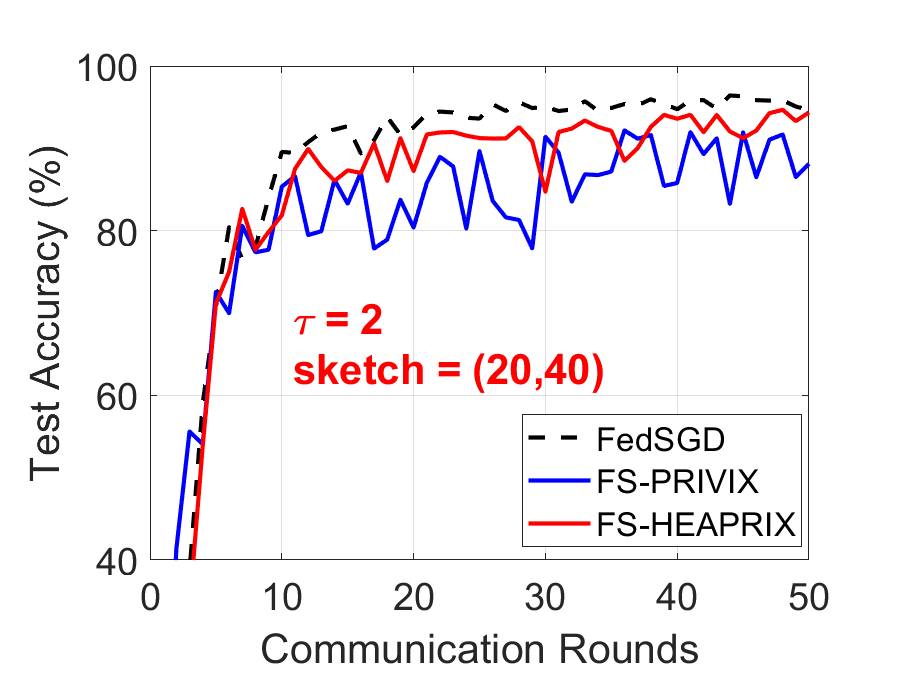
\includegraphics[width=1.6in]{MNIST_figures/local2_sketch20_iid0_test_acc.eps}
% 		\includegraphics[width=1.6in]{MNIST_figures/local2_sketch50_iid0_train_loss.eps}
% 		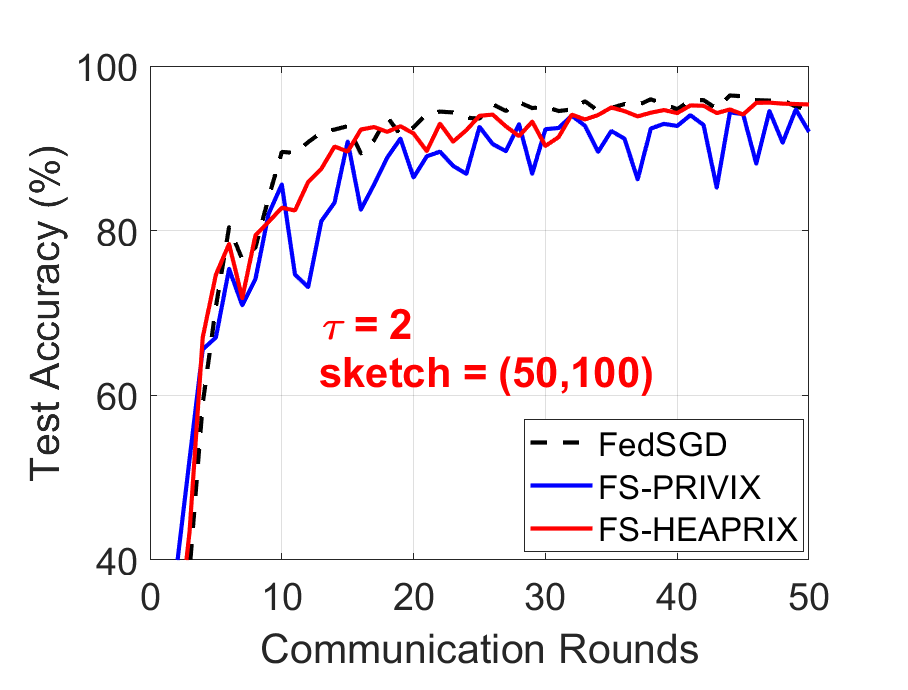
\includegraphics[width=1.6in]{MNIST_figures/local2_sketch50_iid0_test_acc.eps}
% 		}
		
% 		\mbox{			    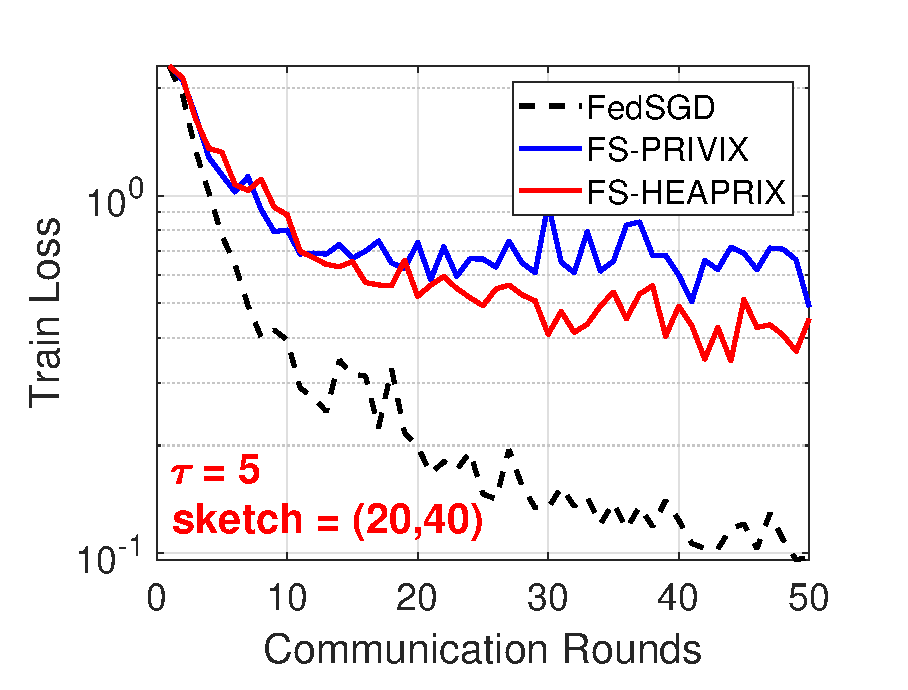
\includegraphics[width=1.6in]{MNIST_figures/local5_sketch20_iid0_train_loss.eps}
% 		\includegraphics[width=1.6in]{MNIST_figures/local5_sketch20_iid0_test_acc.eps}
% 		\includegraphics[width=1.6in]{MNIST_figures/local5_sketch50_iid0_train_loss.eps}
% 		\includegraphics[width=1.6in]{MNIST_figures/local5_sketch50_iid0_test_acc.eps}
% 		}
% 	\end{center}
% 	\caption{Heterogeneous case comparison of FedSGD, FS-PRIVIX and FS-HEAPRIX on LeNet CNN architecture, with number of local updates being 2 and 5.}
%     \label{fig:MNIST-tau2,tau5-iid0}
% \end{figure}

\begin{figure}[h]
	\begin{center}
		\mbox{			    \includegraphics[width=3in]{MNIST_figures/local2_sketch20_iid0_train_loss.eps}
		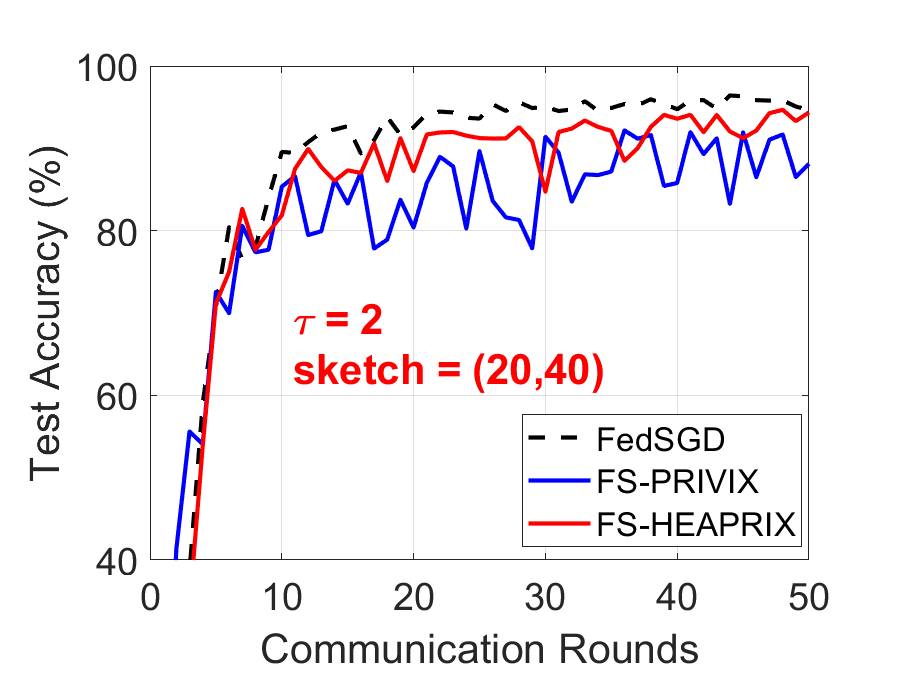
\includegraphics[width=3in]{MNIST_figures/local2_sketch20_iid0_test_acc.eps}
		}
		\mbox{			   
		\includegraphics[width=3in]{MNIST_figures/local2_sketch50_iid0_train_loss.eps}
		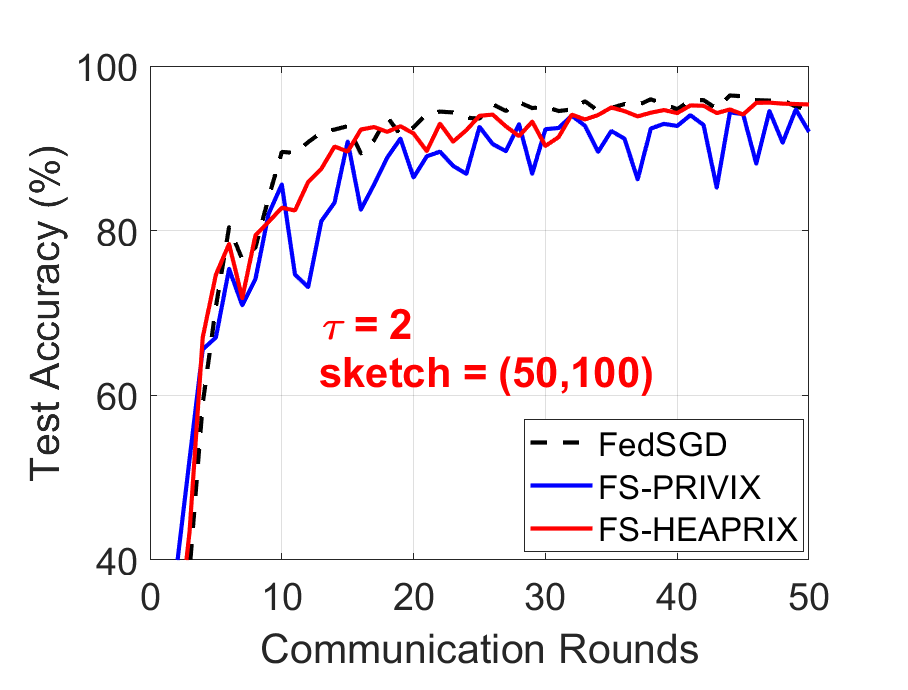
\includegraphics[width=3in]{MNIST_figures/local2_sketch50_iid0_test_acc.eps}
		}
		
		\mbox{			    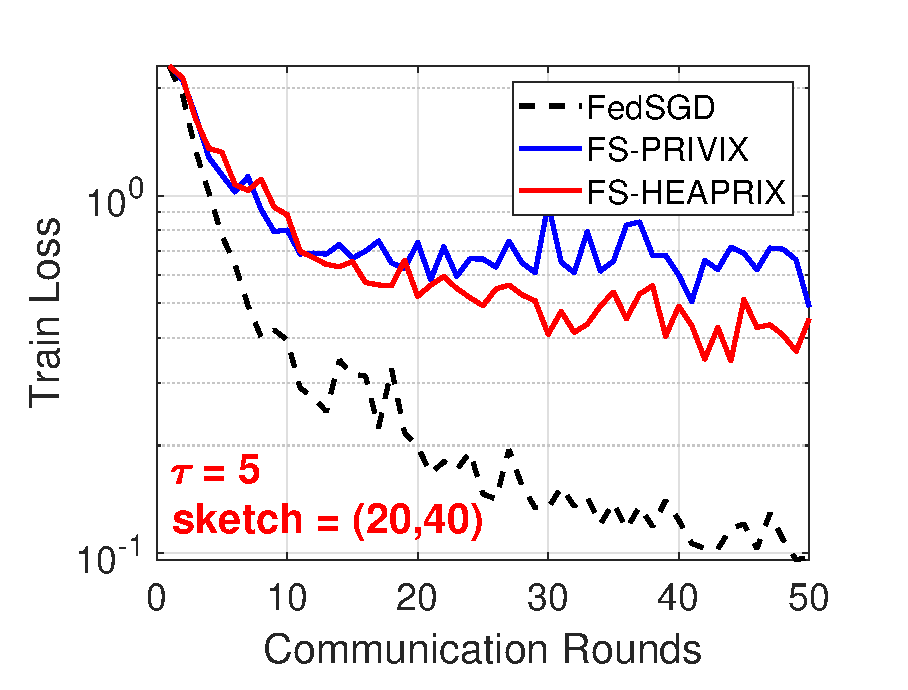
\includegraphics[width=3in]{MNIST_figures/local5_sketch20_iid0_train_loss.eps}
		\includegraphics[width=3in]{MNIST_figures/local5_sketch20_iid0_test_acc.eps}
		}
		\mbox{			   
		\includegraphics[width=3in]{MNIST_figures/local5_sketch50_iid0_train_loss.eps}
		\includegraphics[width=3in]{MNIST_figures/local5_sketch50_iid0_test_acc.eps}
		}
	\end{center}
	\caption{Heterogeneous case comparison of FedSGD, FS-PRIVIX and FS-HEAPRIX on LeNet CNN architecture, with number of local updates being 2 and 5.}
    \label{fig:MNIST-tau2,tau5-iid0}
\end{figure}
